\section{Parte 1. Procesos de Extracción, Transformación y Carga - ETL}

\noindent Como parte de la \underline{descripción del proceso seguido}, y como se ha mencionado anteriormente, fueron utilizadas tres fuentes de datos (Berkeleyn Earth, FAOSTAT, Pinky Rose FIM), de las cuales los datos se encontraban dispersos, con diferencias en su estructura, inconsistencias en su presentación, dificultades en la calidad, entre otros.

\noindent Por parte de \textbf{Berkeley Earth}, fueron obtenidos 164 archivos .txt con información climática correspondiente a 164 países. Al analizar la estructura interna de estos documentos, tomando como caso de estudio el archivo united-states.txt (Estados Unidos), identificamos las siguientes características y retos para su procesamiento
\begin{itemize}
    \item \textbf{Metadatos integrados:} El archivo no inicia directamente con la tabla de datos, sino con un extenso encabezado de texto (comentado con el símbolo \%). Este bloque explica la metodología de medición, indicando que las temperaturas están en grados Celsius y se reportan como anomalías en relación con el promedio histórico del periodo 1951-1980 (para el caso de Estados Unidos). En el proceso ETL, este encabezado debió ser filtrado para poder leer la matriz de datos.
    \item \textbf{Estructura del archivo:} Los datos no están separados por comas (como en un CSV tradicional), sino por espacios en blanco tabulados. La tabla contiene múltiples columnas, de las cuales identificamos como críticas para nuestro modelo: el Año (Year), el Mes (Month), la Anomalía Mensual (Monthly Anomaly) y la Incertidumbre Mensual (Monthly Uncertainty).
    \item \textbf{Problemas de Calidad (Datos Nulos):} El archivo presenta una gran cantidad de datos faltantes registrados bajo la etiqueta NaN (Not a Number), especialmente en los registros históricos más antiguos y en las columnas de promedios suavizados (a 1, 5 o 10 años). Por ello se hizo necesario establecer un rango de tiempo dónde se analizarán los datos, se tomó como punto de partida el año 1990 dónde empiezan los reportes del Pinky Rose y como año de finalización se tomó el año 2015 que es el último reporte de esta base de datos, de esta manera nos eliminamos el problema de los datos etiquetados con NaN.
    
    \begin{figure}[H]
    	\centering
    	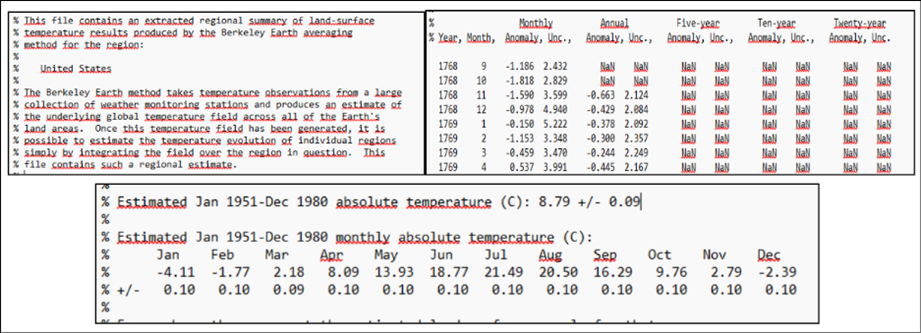
\includegraphics[width=0.8\linewidth]{estructure_berkeley_example.png}
    	\caption{Estructura original del archivo de Berkeley Earth.}
    	\label{fig:berkeley-structure}
    	
    	\vspace{0.2cm}
    	\footnotesize Fuente: Elaboración propia con base en datos de Berkeley Earth.
    \end{figure}
    Para convertir estos datos planos en una tabla estructurada, y poder analizar la información asertivamente, fueron desarrollados los siguientes scripts en Python que denominamos \textbf{01\_country\_name\_mapping.py}, \textbf{02\_download\_berkeley\_files.py} y \textbf{03\_transform\_berkeley\_txt.py} (Scripts ETL), los cuales se encargaron de automatizar la extracción, estructurar el contenido y resolver problemas de calidad de datos: 
\end{itemize}